% 刚体的平面运动方程

\pentry{质心\ 质心系\upref{CM}, 动量定理\upref{PLaw},转动惯量\upref{RigRot}}

任意惯性系中,若刚体质量为 $M$,质心为 $\bvec r_c$,刚体受若干个力 $\bvec F_i$,作用点分别为 $\bvec r_i$,若刚体\bb{只延一个固定的方向转动}(如刚体的二维运动),且该方向关于质心的转动惯量为 $I$, 则质心运动方程和绕质心转动的方程分别为
\begin{equation}\label{RBEM_eq1}
M\bvec a_c = \sum_i \bvec F_i
\end{equation}
\begin{equation}\label{RBEM_eq2}
I \bvec \alpha = \sum_i \bvec \tau_i = \sum_i (\bvec r_i-\bvec r_c) \cross  \bvec F_i
\end{equation}
其中 $\bvec a_c$ 是质心的加速度, $\bvec \alpha$ 是绕质心转动的角加速度.这是说,我们可以把刚体的运动分解成质心的移动和相对质心的转动,并用合力计算前者,用关于质心的合力矩计算后者.

\subsection{推导}
我们把刚体看做质点系来证明,在任意惯性系中,由动量定理,刚体总动量,即质心动量 $\bvec p_c$ 的变化率为
\begin{equation}
\dv{t} \bvec p_c = M \bvec a_c = \sum_i \bvec F_i
\end{equation}

现在我们用角动量定理证明\autoref{RBEM_eq2}.由于质心与刚体的相对位置不变,%未完成:这个怎么证明啊?
质心系中刚体必须绕质心转动,且角动量为(\autoref{RigRot_eq5}\upref{RigRot}) $\bvec L_c = I \bvec\omega$, 角动量变化率为\footnote{注意第一步成立的条件是 $I$ 不变,而一般情况下 $I$ 与刚体的转轴有关,所以只能假设刚体延同一方向转动.唯一的例外是物体的转动惯量与方向无关的情况,例如球体.刚体的变向转动较为复杂,不做讨论.}
\begin{equation}
\dv{\bvec L_c}{t} = I \dv{\bvec \omega}{t} = I \bvec\alpha
\end{equation}
要特别注意的是,除非合力为零,质心系并不是惯性系,所以使用角动量定理要考虑刚体的惯性力.但幸运的是质心系中惯性力(\autoref{Iner_eq5}\upref{Iner}) $-m_i \bvec a_c$ 产生的合力矩为零\upref{PSys}
\begin{equation}
\sum_i \bvec r_{ci}\cross (-m_i \bvec a_{c}) = \bvec a_{c} \cross \sum_i m_i \bvec r_{ci} = \bvec 0
\end{equation}
现在我们可以继续角动量定理\upref{AMLaw} 得
\begin{equation}
I \bvec\alpha = \sum_i \bvec r_{ci} \cross  \bvec F_i
\end{equation}
由于质心系相对于任何惯性系没有相对转动, 所以在任意惯性系中刚体的角加速度仍然为 $\bvec\alpha$.但受力点的位矢变为 $\bvec r_i = \bvec r_c + \bvec r_{ci}$,即
\begin{equation}\label{RBEM_eq7}
I \bvec \alpha = \sum_i (\bvec r_i-\bvec r_c) \cross  \bvec F_i
\end{equation}

\begin{exam}{球体或圆柱延斜面无摩擦滚动}\label{RBEM_ex1}
如\autoref{RBEM_fig1}, 在一个倾角为 $\theta$ 的斜面上, 一个半径为 $R$ 质量为 $M$ 的均匀 的球体(或圆柱)从静止开始向下滚动, 其转动惯量为 $I$, 求质心的加速度和滚动的角加速度.

\begin{figure}[ht]
\centering
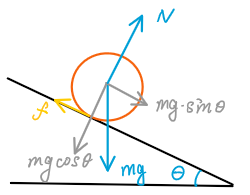
\includegraphics[width=5.3cm]{./figures/RBEM1.png}
\caption{圆柱延斜面无摩擦滚动} \label{RBEM_fig1}
\end{figure}

解: 首先, 根据无摩擦的条件, 系统只有一个自由度\upref{DoF}, 即圆柱的位移或者转角, 二者的关系为
\begin{equation}
s = R\theta
\end{equation}
两边求二阶导数, 得加速度与角加速度的关系为
\begin{equation}\label{RBEM_eq3}
a = R\alpha
\end{equation}

受力分析如图, 圆柱受三个力: 重力, 支持力和静摩擦力. 将物体受到的重力分解为垂直斜面方向和沿斜面方向的两个分力. 其中垂直方向的分力与斜面提供的支持力抵消, 而平行方向的分量和摩擦力的合力决定质心的加速度\autoref{RBEM_eq1}
\begin{equation}\label{RBEM_eq4}
mg\sin\theta - f = Ma
\end{equation}
再来分析关于质心的转动, 由于重力和摩擦力都在质心, 所以对合力矩贡献为 0. 所以只有摩擦力的贡献为 $\tau = fR$, 由\autoref{RBEM_eq2} 得
\begin{equation}\label{RBEM_eq5}
I\alpha = f R
\end{equation}
由\autoref{RBEM_eq3}到\autoref{RBEM_eq5} 三式解得加速度为
\begin{equation}
a = \frac{g \sin\theta}{1 + I/(MR^2)}
\end{equation}
可见转动惯量为 0 时, 结果与无摩擦滚动一致. 而转动惯量越大, 加速度就越小.
\end{exam}

\begin{exam}{}
一根质量为 $M$ 长为 $L$ 的均匀细棒延 $y$ 方向静止放置在水平面 $xy$,从 $t=0$ 时起在其上端施加一个 $x$ 方向的恒力,描述细棒如何运动.如果木棒与地面的摩擦系数为 $\mu$,答案又如何?

首先考虑质心的运动, 细棒所受外力只有一个恒力, 所以由\autoref{RBEM_eq1} 质心沿 $x$ 方向做匀加速运动. 再来看质心系中细棒的转动由“ 转动惯量\upref{RigRot}” 中\autoref{RigRot_ex1} 可知细棒绕其质心做单摆运动.
% 未完成: 分析有摩擦的情况
\end{exam}
